\chapter{Results and Discussion}
\section{Virtual Prototyping of Cell Signals}
\label{sec:res:simMag}
During the course of this thesis, numerical simulations for the microchannel have been carried out in MATLAB. First, a simulation about the shape of a \gls{gmr}-sensor signal of cells was performed, where the magnetic moment was conveyed through \glspl{mnp} bound to their surface. Second, cell aggregates have been looked at in the same manner with different angles respective to the sensor. Third, both simulations were correlated to a reference dipole, with the equivalent magnetic moment located in the center of mass.\\
Additionally, the flow and shear field inside the channel was simulated numerically for the channel cross-section as well as for a particle near the walls. A force equilibrium simulation was also established in a basic manner. \\
All simulations have been captured inside the MATLAB class ``MRCyte'', which contains material parameters, constants, and the necessary functions for all simulations above.
\subsection{Numerical investigation of immunomagnetic label density and size on quantitative magneto-resistive sensing of single cells and cell aggregates}
In order to mimic an immunomagnetically labeled cell flowing over the sensor half-bridge, the planar integral of the respective \acrfull{B} was solved analytically. Here, $\mathbf{r}_i$ specifies the distance vector of a single \gls{mnp} from the sensor plane. The magnetic flux density was converted to a resistive change $\mathbf{R}_\text{sig}$ by scaling it with the \gls{gmr}-sensitivity $S$ and subsequently into a signal voltage $\mathbf{V}_\text{sig}$ inside the bridge branch.(\cref{eq:magneticFluxIntegral,eq:GMR-signal,eq:voltage-signal})\\
\begin{align}
	\mathbf{B}(t) &= \sum_{i=1}^{N} \frac{1}{A_{\text{Sensor}}} \int_{-\frac{l}{2}}^{\frac{l}{2}} \int_{-\frac{w}{2}}^{\frac{w}{2}} \frac{\mu_{o}}{4 \pi}\left(\frac{3 \mathbf{r}_{i}(t)\left(\mathbf{r}_{i}(t) \cdot \mathbf{m}_{i}\right)}{\left|\mathbf{r}_{i}(t)\right|^{5}}-\frac{\mathbf{m}_{i}}{\left|\mathbf{r}_{i}(t)\right|^{3}}\right) \text{dx dy} \label{eq:magneticFluxIntegral} \\
	\mathbf{R}_\text{sig}(t) &= - \mathbf{B}(t) \times \frac{S}{100} \times R + R \label{eq:GMR-signal}\\
	\mathbf{V}_\text{sig}(t) &= \frac{\mathbf{R}_\text{sig}(t)}{R + \mathbf{R}_\text{sig}(t)}\times V_\text{p} - \frac{V_\text{p}}{2} \label{eq:voltage-signal}
\end{align}
First, \glspl{mnp} were randomly sampled on a sphere surface with a diameter of \SI{4}{\micro\meter} or \SI{8}{\micro\meter}. Then, the signal was computed from the superposition of every \gls{mnp} during each timestep. Additionally, the \gls{mnp} distribution was rotated in every iteration to resemble a rolling motion. The computed signals were then cross-correlated to the signal of a reference flux density $\mathbf{B}_\text{ref}$ caused by a point-like magnetic moment located in the geometric center of the same sphere.
By its formula, cross-correlation $R_\text{x y}(\tau)$ yields a displacement dependent signal through its convolution of the complex conjugated reference signal $\mathrm{V}_\text{ref}^{*}(t)$ with the sample signal $\mathbf{V}_\text{sig}(t+\tau)$.(\cref{eq:xcorr}) Therefor, only the maximal correlation of this function was considered in further analyses.
\begin{equation}
	\mathrm{max}\{R_\text{x y}(\tau)\}=\mathrm{max}\left\{\int \mathrm{V}_\text{ref}^{*}(t) \mathbf{V}_\text{sig}(t+\tau) \text{dt} \right\} \label{eq:xcorr}
\end{equation}
\begin{figure}[ht!]
	\centering
	\begin{minipage}[t]{.24\linewidth}
		\subfloat{
			\subfigimg[height=323pt]{a}{Ressources/Simulation/GMR}			
			\phantomsubcaption
			\label{fig:sim:intro:gmr}
		}
	\end{minipage}%
	\hfill
	\begin{minipage}[b]{.7\linewidth}
		\addtocounter{subfigure}{-1}
		\subfloat{
			\subfigimg[width=\linewidth]{b}{Ressources/Simulation/ParticleCoverage}
			\phantomsubcaption
			\label{fig:sim:intro:coverage}
		} 
		\\
		\vspace{\baselineskip}	
		\addtocounter{subfigure}{-1}
		\subfloat{
			\subfigimg[width=\linewidth]{c}{Ressources/Simulation/ParticleAngle}			
			\phantomsubcaption
			\label{fig:sim:intro:angle}
		}
	\end{minipage}%	
	\capption{Particle Coverage Simulation}{(\textbf{a}) Dimensions of the \gls{gmr} Wheatstone bridge sensor: Distance d between both variable bridges (green), width w of a \gls{gmr}-sensor, length L of a sensor. (\textbf{b}) Scheme of single-cell simulation: The ideal magnetic dipole in the geometric center of a sphere (\blueCircle) causes a signal deviation from the real cell signal with magnetic moment distributed on the cell surface. (\orangeCircle) (\textbf{c}) Signal shapes of different angles of two-particle aggregates lead to differing signal shapes. }
	\label{fig:sim:intro}	
\end{figure}

\subsection{Single-Cell Signals}
The aim of these simulations is to find a measure of how magnetic labeling of a cell affects its signal shape and subsequent analysis. A single cell with a surface coverage of \SIrange{5}{99}{\percent} of a densely packed sphere was loaded randomly with \glspl{mnp} of different sizes. Then, the previously explained rolling motion over the sensor bridge was simulated with the parameters specified in \cref{tab:params:mag_sim}. After correlating of the resulting signal voltage to the reference dipole (\cref{fig:sim:intro:coverage}, \blueCircle), each with three equal, randomly distributed \gls{mnp} coverages, the dependency on the coat was evaluated. As shown in the schematic \cref{fig:sim:intro:coverage}, an increase in signal peak amplitude but also in \gls{fwhm} at growing coverage was expected. 
\begin{figure}[!h] 	
	\centering
	\subfloat{	
		\subfigimg[height=150pt]{a}{Ressources/Simulation/Small2um}	
		\phantomsubcaption
		\label{fig:sim:coverage:small2um}
	} \hfill
	\addtocounter{subfigure}{-1}
	\subfloat{
		\subfigimg[height=150pt]{b}{Ressources/Simulation/Big2um}
		\phantomsubcaption
		\label{fig:sim:coverage:big2um}	
	} \\
	\vspace{\baselineskip}	
	\addtocounter{subfigure}{-1}
	\subfloat{	
		\subfigimg[height=150pt]{c}{Ressources/Simulation/Small4um}	
		\phantomsubcaption
		\label{fig:sim:coverage:small4um}
	}\hfill
	\addtocounter{subfigure}{-1}
	\subfloat{
		\subfigimg[height=150pt]{d}{Ressources/Simulation/Big4um}
		\phantomsubcaption
		\label{fig:sim:coverage:big4um}
	}
	\capption{Coverage Dependent Signal Correlation}{\gls{mnp} coverage of a sphere with \SI{4}{\micro\meter} (\textbf{a}, \textbf{b}) and \SI{8}{\micro\meter}  diameter  (\textbf{c}, \textbf{d}) covered by magnetic particles ranging from \SIrange{20}{2000}{\nano\meter}. A cross-correlation increase which is inversely proportional to the \gls{mnp} size can be observed.}
	\label{fig:sim:coverage}
\end{figure}
\clearpage
The expected behavior matches the data analysis (\cref{fig:sim:coverage}). Each two analyzed sphere diameters \SIlist{4;8}{\micro\meter} with \gls{mnp} sizes ranging from \SI{20}{\nano\meter} to \SI{2}{\micro\meter}, show a great \gls{sem} at low coverage. This very probably is subjected to the momenta of single particles which play a greater individual role and hence influence the signal shape significantly because the overall dipole moment in the sensor loses homogeneity. \\
Another observable effect is related to the \gls{mnp} size. Absolute correlation differs from \SI{20}{\nano\meter} to the ten and hundred-fold diameter significantly. This can be related to the magnetic moment per \gls{mnp} as it is dependent on the volume - thus $r^3$.

However, for bigger magnetic particles this does not completely hold because the composition changes from pure magnetite to a polymer shell with embedded oxide core at around \SI{150}{\nano\meter}. Nevertheless, larger particles carry also greater magnetic moment which brings the aforementioned influence of single \glspl{mnp} into consideration. \\ 
Further, the densely packed sphere surface can carry substantially more smaller than larger \glspl{mnp}. This ranges from \num{641600} \gls{mnp} of \SI{20}{\nano\meter} to \num{81} of \SI{2}{\micro\meter} for a sphere radius of \SI{4}{\micro\meter} and thus limits the maximum achievable moment. \\
In reality, a maximum immunomagnetic label density depends not on the densely packed sphere but rather on the present antigens, and association or dissociation constants. Therefore, a complete saturation coverage is not achievable under physiological conditions. When using smaller particle sizes, it has to be taken into consideration that a cumulative magnetic moment is limited by the number of antigens and the detection limit of the sensing setup.
\begin{align}
	\text{Relative\ Correlation\ Difference} &= 1- \frac{\max\{\text{Cross-Correlation}(d=\SI{4}{\micro\meter})\}}{\max\{\text{Cross-Correlation}(d = \SI{8}{\micro\meter})\}} \label{eq:sim:relCorrDiff}\\
	\text{Relative\ Correlation\ Difference} &= \num{-0,38532} \, {d_\text{MNP}}^2 + \num{3,34574} \, d_\text{MNP} - \num{8,49629} \label{eq:sim:quadFit}
\end{align}
Also, it can be seen that the correlation approaches a maximum obtainable value for every \gls{mnp} size. Referenced for both simulated sphere diameters in \cref{fig:sim:CorrDiff:abs}, an inverse proportionality between correlation and \gls{mnp} diameter is visible. The trend in respective maxima can be attributed to variations in the magnetic moment, and coverage inhomogeneity. \clearpage
Inter-sphere compared, maximum correlation shows also a significant deterioration for higher \gls{mnp} sizes as the particle diameter itself increases. The relative error between both sizes - as computed in \cref{eq:sim:relCorrDiff} -  is depicted in \cref{fig:sim:CorrDiff:rel}. Assuming a dependency on the available particle surface and subsequently the fraction which can be occupied by \glspl{mnp}, a quadratic fit seems appropriate.(\cref{eq:sim:quadFit}) The fit indicates probably that a cell covered with small \glspl{mnp} resembles a magnetic dipole located in the center of the cell while the correlation error becomes nearly constant at great \glspl{mnp}.


\begin{table}[h!]
	\centering
	\begin{tabularx}{\linewidth}{cccc}
		\toprule[1pt]
		\rule[-1ex]{0pt}{2.5ex} Parameter & Unit & Value & Explanation \\	
		\midrule
		\rule[-1ex]{0pt}{2.5ex} w & \si{\meter} & \num{2.0e-6} & GMR width \\
		\rule[-1ex]{0pt}{2.5ex} l & \si{\meter} & \num{30.0e-6} & GMR length \\
		\rule[-1ex]{0pt}{2.5ex} d & \si{\meter} & \num{14.0e-6} & Distance between two sensors \\
		\rule[-1ex]{0pt}{2.5ex} $R$ & $\mathrm{\Omega}$ & 250 & GMR Resistance\\
		\rule[-1ex]{0pt}{2.5ex} \gls{el:vp} & \si{\milli\volt} & 100 & Supply voltage\\
		\rule[-1ex]{0pt}{2.5ex} t$_\text{free\ layer}$ & \si{\meter} & \num{7.0e-9} & Thickness of free layer\\
		\rule[-1ex]{0pt}{2.5ex} $\mathbf{M}$ & \si{\ampere\per\meter} & \num{2.0e4} & Volume Magnetization\\
		\rule[-1ex]{0pt}{2.5ex} $V_\text{noise,rms}$ & \si{\volt} & \num{2.5e-6} & Artificial noise\\
		\rule[-1ex]{0pt}{2.5ex} Sim. Space & \si{\meter} & [\num{-25e-6},\num{25e-6}] & Interval around sensor center \\	
		\bottomrule[1.2pt]
	\end{tabularx}
	\capption{Magnetic Simulation Parameters}{Constants used inside the framework for the simulation of the magnetic field inside the \gls{gmr} Wheatstone half-bridge. The volume magnetization was adapted according to the simulated particle size.}
	\label{tab:params:mag_sim}
\end{table}
\clearpage
\subsection{Cell Aggregates}
In another simulation, two \SI{200}{\nano\meter}-\gls{mnp}-covered spheres were attached in different angles and simulated flowing over the sensor. Signal similarity to a magnetic dipole in the center of a single reference sphere was computed by cross-correlation. As can be observed in \cref{fig:sim:aggregates}, correlation is identical to a single sphere at low coverage, above a threshold magnetization. Here, the randomly distributed particles span an inhomogeneous magnetic field of a larger sphere which cannot be subdivided into the two singular parts.\\
With growing coverage, each cell starts to form an independent dipole. At occupancies greater than \SI{50}{\percent}, the two attached cells are in such superposition. Now, the sensor detects not a single particle as for less coverage but two spatially close particles. Consequentially, the signal is an interference pattern of the two singular events and thus carries small peaks in the center. This is shown schematically in \cref{fig:sim:intro:angle}. In term, this causes a high signal deviation from the reference and a low degree of correlation effectively.
\clearpage
\begin{figure}[h!]
	\centering
	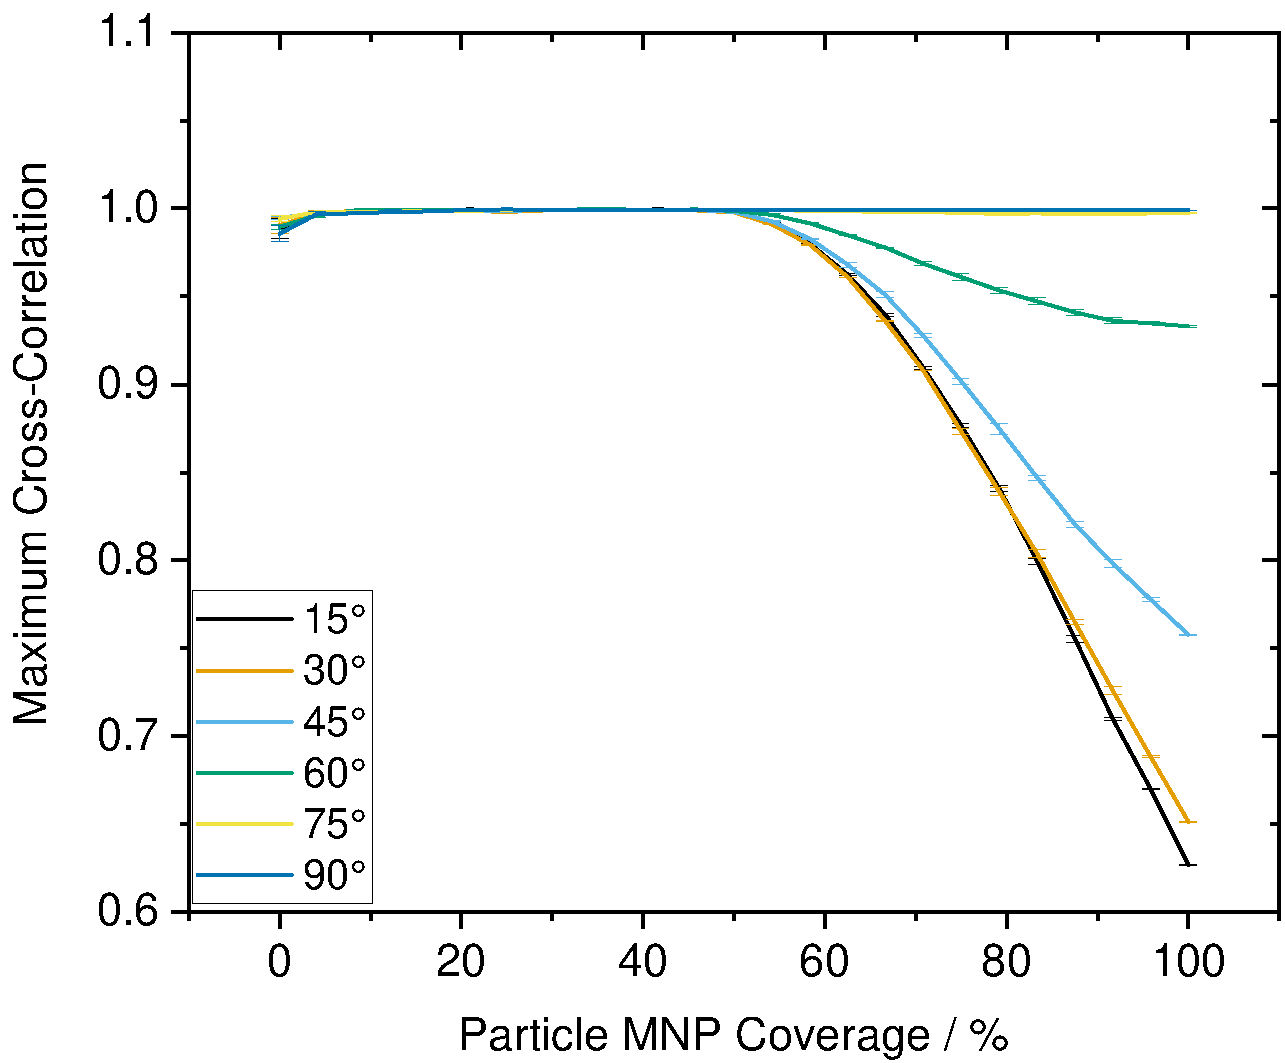
\includegraphics[width=.7\linewidth]{Ressources/Simulation/Aggregates}	
	\capption{Signal Correlation between Two-Cell Aggregates At Shifting Angles}{Two-Sphere aggregates are covered with \SI{200}{\nano\meter} \glspl{mnp} and simulated flowing over the sensor at differing respective angles. The \gls{sem} indicates a difference in the cross-correlation of three truly random \gls{mnp} distributions. For low yaw angles and high coverages, the aggregate's signal reflects rather two single dipoles in superposition than one quite homogeneous dipole. This causes a high signal deviation from the reference and thus a low degree of correlation.}
	\label{fig:sim:aggregates}
\end{figure}
\begin{figure}[h!]
	\centering
	\subfloat{
		\subfigimg[height=150pt]{a}{Ressources/Simulation/CrossCorr-Maximal}
		\phantomsubcaption
		\label{fig:sim:CorrDiff:abs}	
	} \hfill
	\addtocounter{subfigure}{-1}
	\subfloat{
		\subfigimg[height=150pt]{b}{Ressources/Simulation/CrossCorr-Error}	
		\phantomsubcaption
		\label{fig:sim:CorrDiff:rel}
	}
	\capption{Maximal Cross-Correlation Differences}{(\textbf{a}) Mean coverage at \SI{99}{\percent} for \SI{4}{\micro\meter}  and \SI{8} {\micro\meter} spheres. A negative dependency on the \gls{mnp} size can be explained by the ratio of magnetic moment per unit surface and its homogeneous distribution across the whole surface.\\ (\textbf{b}) Relative correlation error between \SI{4}{\micro\meter}  and \SI{8} {\micro\meter} spheres with a quadratic fit. The quadratic behavior could be related to the relative surface area which can be occupied by magnetic moment. (Adj. $R^2$ = \num{0.99209})}
	\label{fig:sim:CorrDiff}
\end{figure}
\clearpage

\section{The MRCyte Simulation Framework}
In this work, also an analytical simulation framework that is capable of simulating the synergy of multiple microfluidic effects was developed. The comprehensive framework features magnetic, fluid dynamic, and biochemical processes inside the utilized microfluidic channel which act on a particle. Foremost, material parameters were stored inside the ``MRCyte'' class, which ranged from channel and particle properties to binding and friction constants. Basic velocity, shear, and magnetic field computations build the core of the presented program. Additionally, several dimensionless parameters such as the Stokes or \gls{re} or particle properties can be computed.\\
With that, simulations of the fluid dynamics that influence a single microbead as well as force-equilibrium computations for the same bead were carried out. 
%\todo{Capabilities - Simulation bead over sensor, particle distribution on surface, analysis of GMRTool data single and differential, magnetic field permanent}

\subsection{Fluid Fields inside the Microchannel}
\label{sec:res:fluidSim}
The simulation framework provided a quantitative generation of the Hagen-Poiseuille flow profile inside the microchannel with the numerical solution of \cref{eq:flowRateRect}. The simulated channel had dimensions (\gls{chanW} $\times$ \gls{chanH} $\times$ \gls{chanL}) \SI{700}{\micro\meter} $\times$ \SI{150}{\micro\meter} $\times$ \SI{15800}{\micro\meter}. The flow rate was adopted to \SI{80}{\micro\liter\per\minute}.\footnote{in accordance with the experimentally determined value} Tubing as well as time-dependent effects were neglected. \\
The simulated \gls{u} for the whole channel cross-section can be observed in \cref{fig:sim:flowShear:vel:full}. Due to the no-slip boundary condition, \gls{u} is zero on the margin while the maximum of is reached in the geometric center. \gls{umean} in the channel ensues \SI{12670.84}{\micro\meter\per\second}.\\
Conjointly, computation of the flow gradient in a vertical direction and scaling with \gls{eta} yield the shear stress field.(\cref{fig:sim:flowShear:shear:full}) As the curvature of \gls{u} is zero in the channel center and maximal at the edges, the shear stress reaches its largest values symmetrically at the horizontal edges of the channel.\footnote{Because the horizontal components of the gradients were neglected graceless} Resulting, the net viscous shear $\boldsymbol{\tau}_\text{viscous} = \frac{\partial u}{\partial z}$ cancels out over the whole channel cross-section.

Additionally, \gls{u} and \gls{tau_v} acting on an \SI{8}{\micro\meter} diameter bead on the channel bottom were analyzed.(\cref{fig:sim:flowShear:vel:particle,fig:sim:flowShear:shear:particle}) In the proximity of a wall and due to the applied boundary conditions, \gls{tau_v} enclosed by the bead surface is non-linear. Thus, the mean fluid velocity exposed to the bead amounts in $\overline{\mathbf{u}_\text{p}}$ =  \SI{2241.59}{\micro\meter\per\second}, whereas  $\overline{\boldsymbol{\tau}_\text{viscous,\, p}}$ strains with \SI{4.93}{\dyne\per\square\centi\meter}.

\begin{figure}[htb!]
	\centering	
	\subfloat{
		\subfigimg[height=135 pt]{a}{Ressources/Simulation/Flow/150um_vel}	%[width=\linewidth
		\phantomsubcaption
		\label{fig:sim:flowShear:vel:full}
	} \hfill
	\addtocounter{subfigure}{-1}
	\subfloat{
		\subfigimg[height=135 pt]{b}{Ressources/Simulation/Flow/150um_vel_particle}			
		\phantomsubcaption
		\label{fig:sim:flowShear:vel:particle}
	} \\
	\addtocounter{subfigure}{-1}
	\vspace{\baselineskip}
	\subfloat{
		\subfigimg[height=135 pt]{c}{Ressources/Simulation/Flow/150um_shear_chan}					
		\phantomsubcaption
		\label{fig:sim:flowShear:shear:full}
	} \hfill
	\addtocounter{subfigure}{-1}
	\subfloat{
		\subfigimg[height=135 pt]{d}{Ressources/Simulation/Flow/150um_shear_part}					
		\phantomsubcaption
		\label{fig:sim:flowShear:shear:particle}
	}
	%	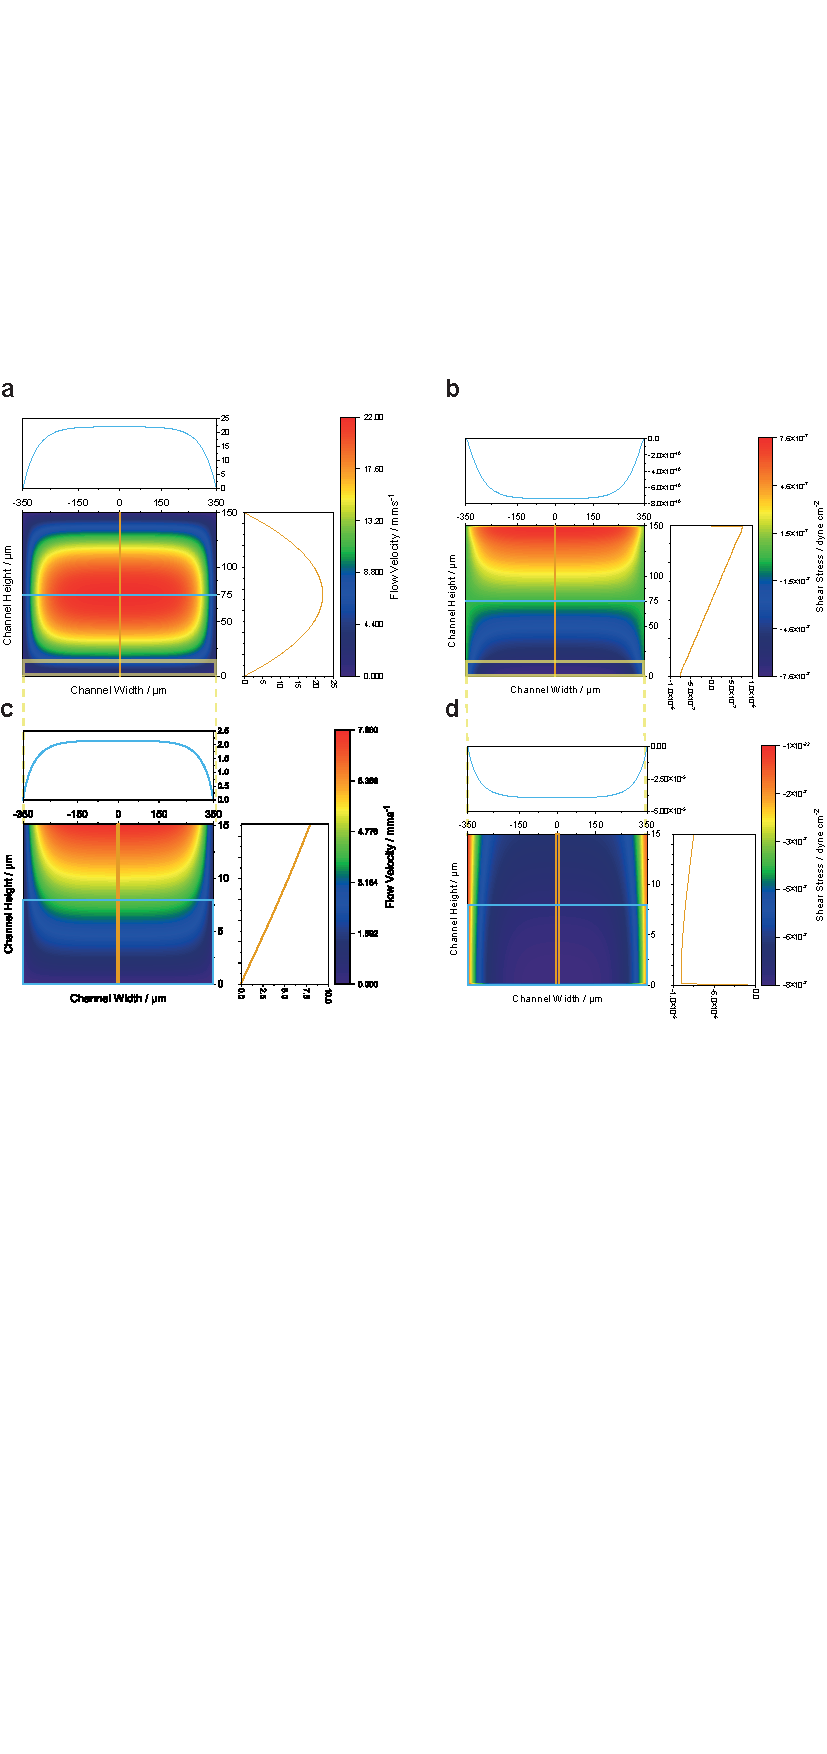
\includegraphics[width=\linewidth]{Ressources/Simulation/FlowShearFigure}
	\capption{Flow Field and Shear Stress Simulation of the utilized Microchannel}{Flow (\textbf{a}) and vertical shear (\textbf{c}) field inside the microchannel with dimensions (\gls{chanW} $\times$ \gls{chanH} $\times$ \gls{chanL}) \SI{700}{\micro\meter} $\times$ \SI{150}{\micro\meter} $\times$ \SI{15800}{\micro\meter} for a flow rate of \SI{80}{\micro\liter\per\minute} and with neglected tubing effects. The subplots on the right and top sides show the mean horizontal and vertical profile in \SI{0}{\micro\meter} width and \SI{75}{\micro\meter} height, respectively. (vertical: \blueline, horizontal: \orangeline) Due to the no-slip condition, the velocity at the walls equals zero and the shear is maximal. The maximum of the Hagen-Poiseuille profile is located in the channel center. Over the cross-section the mean flow velocity $\overline{\mathbf{u}}$ equals \SI{12670.83}{\micro\meter\per\second}. Resultingly, the net horizontal viscous shear  $\boldsymbol{\tau}_{viscous} = \frac{\partial u}{\partial z}$ cancels out over the whole channel cross-section. \\
	Flow (\textbf{d}) and vertical shear (\textbf{d}) field acting on an \SI{8}{\micro\meter} diameter bead on the channel bottom. The mean fluid velocity trapped by the bead profile results in  $\overline{\mathbf{u}_{p}}$= \SI{2241.59}{\micro\meter\per\second}, whereas the viscous shear strains with $\boldsymbol{\tau}_{viscous}$ = \SI{4.93}{\dyne\per\square\centi\meter} }
	\label{fig:sim:flowShear}
\end{figure}
\clearpage

\subsection{Modeling the Force-Equilibrium of a Rolling Bead over a Biofunctionalized Surface}
\label{sec:res:forcesim}
With the supplier's parameters of an \SI{8}{\micro\meter} micromer-M bead (micromod Partikeltechnologie GmbH, Rostock) the corrected drag force on a bead on the bottom of the standard utilized microchannel results in \SI{463.65}{\pico\newton} for \SI{80}{\micro\liter\per\minute}. This is computed from \cref{eq:f:drag} and the correction factor in \cref{eq:f:drag:corr:wall_approx}, where the simulated flow field integrated over the particle surface was plugged into.\\
If the bead was functionalized with biotin under the negligence of the corresponding differential equations for association constants, the number of interacting groups would result in the present surface charges. Surface charge density results in \SI{1}{\micro\mole\per\gram} of \gls{carboxyl} and \gls{amine} beads as of the supplier's data sheet. Hence, a fully saturated bead is covered with \num{177500} biotin molecules.\\
The streptavidin coverage of the channel floor was modeled in excess over the biotin ligands and penetration depth was estimated by the size of several monolayers of protein. As described by \citet{lit:fluidic:ModelMIT}, an approach of \SI{30}{\nano\meter} is a reasonable quantity. In turn, the surfaces were in contact with \SI{1.51}{\micro\meter\squared} which constitutes \SI{0.75}{\percent} of the \SI{8}{\micro\meter} bead surface. This reveals that \num{1329} biotin molecules can interact with the floor. A summation of the \gls{f:protein} at \SIrange{5}{150}{\pico\newton} per streptavidin-biotin bond yields the resulting adhesion force with a magnitude of \SIrange{6.7}{199}{\nano\newton}.\cite{lit:bio:biotin:rupture} 

The binding force is in the same range as the perpendicular magnetophoretic force caused by the permanent magnet under the sensor chip ($\nabla \mathbf{B}$ = \SI{10}{\tesla\per\meter}) as well as by the nickel-iron chevron structures on the chip ($\nabla \mathbf{B}$ $\approxeq$ \SI{5}{\kilo\tesla\per\meter}). Clearly, in the near-field approximation, the nickel-iron structures dominate \gls{f:mag} (\cref{eq:f:mag}). With the manufacturer declared saturation moment of one particle (\SI{1.12}{\pico\ampere\meter\squared}), the magnetic attraction force eventuates in \SI{5.6}{\nano\newton} in the magnetophoresis section of the channel.
\begin{align}
	\mathbf{F}_\parallel = \mathbf{F}_\text{drag} - C_\text{rr} \cdot (\mathbf{F}_\text{mag} \ +\ \mathbf{F}_\text{protein}  \ +\ \mathbf{F}_\text{grav}\ -\ \mathbf{F}_\text{shear} ) \label{eq:f:balance} \\
	C_\text{rr} = \sqrt{\frac{\text{z}}{d}} = \sqrt{\frac{\SI{30}{\nano\meter}}{\SI{8}{\micro\meter}}} = \num{0.0612} \label{eq:corr:roll}
\end{align}
\clearpage
In order to merge this analytic force balance, all remaining forces have to be projected into the direction of \acrfull{f:drag}.(\cref{eq:f:balance}) This is achieved by the introduction of a \gls{corrRoll} for a perfectly elastic surface.(\cref{eq:corr:roll}) In a first-order approximation, the factor depends only on the \acrfull{z} and the bead diameter ($d$). However, scientific literature about the rolling resistance of microbeads on microfluidic or protein-covered surfaces does not exist yet to confirm this macroscopic factor for the microscale. \\
Scaling all orthogonal forces to the \acrlong{f:drag} with \gls{corrRoll} yields a net positive result (\SI{154.08}{\pico\newton}) for an unfunctionalized surface (\gls{f:protein} $\overset{!}{=}$ \num{0}) which indicates a rolling motion in the flow direction. Notwithstanding, above a critical interaction number of \numrange{503}{16} biotin-streptavidin bonds - for the respective release forces of \SIrange{5}{150}{\pico\newton} per linkage - the particle resists \acrlong{f:drag} and adheres to the surface.

This behavior will be exploited in further measurements for ``bead loss experiments'' in order to measure a concentration difference with different degrees of biotinylated beads.


\clearpage
\section{Reference Bead Surface Functionalization}
\label{sec:res:beadFunc}
After simulation of their respective coverages, biotin was titrated on \SI{8}{\micro\meter} reference beads with two different surface terminations in order to selectively bind \glspl{mnp} with the counter-agent streptavidin to the surface. First, \gls{amine}-microbeads were modified by sulfo-NHS-biotin. Second, \gls{carboxyl} beads were coated by amine-PEG$_2$-biotin via EDC-NHS-activation. On the same beads, Anti-IgG1-PE antibodies were titrated after the same coupling chemistry.\\
Subsequently, biotin-coated beads were analyzed in the flow cytometer in the by a stain with Atto-488 (Ex: \SI{500}{\nano\meter}, Em: \SI{520}{\nano\meter}) coupled streptavidin. The antibody was modified with \gls{pe} and measured at \SI{488}{\nano\meter} excitation and \SI{585}{\nano\meter}  emission wavelength. The gating was standardized by the strategy found in \cref{sec:meth:beadCharact}, \cref{fig:gatingstrategy-layout}. Subsequently, the \gls{mfi} was computed and fitted with a sigmoidal Hill-function.(\cref{eq:hill}) The Stability of carboxylated and aminated beads and subsequently their respective modification protocols were evaluated for \SI{12}{days}.


\subsection{Amine-Surface Biotinylation}
As a first approach, polystyrene copolymer microbeads with \SI{8}{\micro\meter} diameter were functionalized by (sulfo-)NHS-biotin after a standard protocol from Thermo Fisher Scientific and micromod. A titration of the biotin reactant yielded a varying surface coverage as shown in \cref{fig:biotinyl:titration:nh2}. During this one-pot-reaction, the water-soluble sulfo-NHS-biotin forms an \gls{amide} linkage with the primary \gls{amine} and \iupac{1-\-hydroxy\--2,5-\-dioxo\-pyrrolidine-\-3-\-sulfonate} splits off as a byproduct.\\
As can be seen from the \gls{sem} error bars from plot \ref{fig:biotinyl:titration:nh2}, which were obtained from three true biological replicates, this process is highly reproducible. Therefore, surface coverage in different grades of biotinylation could be incurred accurately with an \gls{rsquadj} of \num{0.981} for the resulting Hill fit.

\begin{figure}[h]
	\centering
	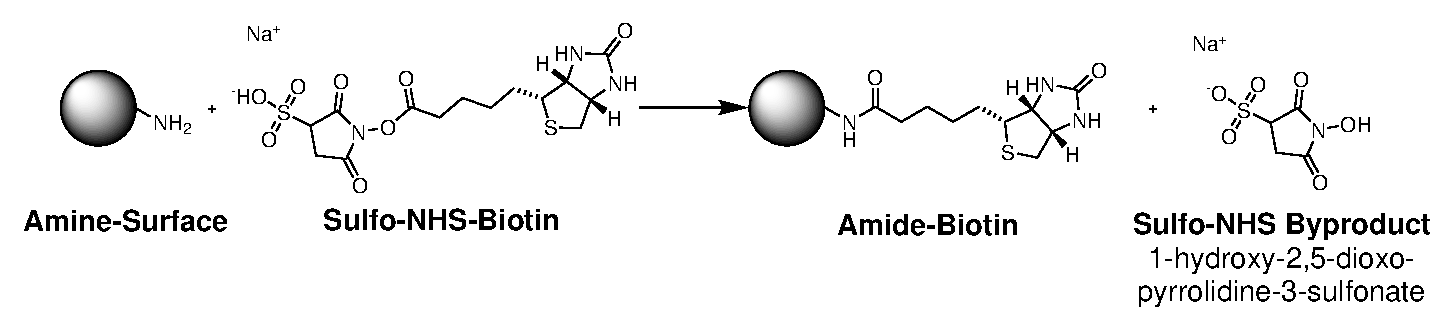
\includegraphics[width=\linewidth]{./Ressources/Chemistry/Sulfo-NHS.eps}
	\capption{Amine Bead Modification with Sulfo-NHS-Biotin}{An amine-terminated bead is brought into reaction with sulfo-NHS-biotin. Both form an amide linkage and bind biotin covalently to the surface. As a byproduct the sulfo-NHS-ester splits off.}
	\label{fig:Chem:NH2-NHS}
\end{figure}

\clearpage

\begin{figure}
	\centering
	\subfloat{
		\subfigimg[height=95pt]{a}{./Ressources/Biotinyl/mag-nh2}	
				\phantomsubcaption
		\label{fig:biotinyl:titration:nh2}
	} \hfill
	\addtocounter{subfigure}{-1}
	\subfloat{
		\subfigimg[height=95pt]{b}{./Ressources/Biotinyl/cooh}	
		\phantomsubcaption
		\label{fig:biotinyl:titration:cooh}
	}\hfill
	\addtocounter{subfigure}{-1}
	\subfloat{
		\subfigimg[height=95pt]{c}{./Ressources/Biotinyl/IgG-cooh}	
		\phantomsubcaption
		\label{fig:biotinyl:titration:igg}
	} \\
	\addtocounter{subfigure}{-1}
	\vspace{\baselineskip}
	\subfloat{
	\subfigimg[width=.7\linewidth]{d}{./Ressources/Biotinyl/stability}
	\phantomsubcaption
	\label{fig:biotinyl:titration:stability}	
	}

	\capption{Titration of Biofunctional Molecules on \SI{8}{\micro\meter} Particles}{ Titration curves of NHS-biotin (\textbf{a}), Amin-PEG$_2$-Biotin (\textbf{b}), and Anti-IgG1 (\textbf{c}) with their respective Hill fits. The corresponding fit parameters, as well as the goodness factor, are shown in \cref{tab:biotinyl:fitParams:beads}. (\textbf{d}) Stability analysis of functionalized \gls{carboxyl} and \gls{amine} beads over \SI{12}{days}. The carboxylate particles show an exponential decrease with a half-life of \SI{1.43}{days} as determined by the exponential fit. The respective parameters are shown in \cref{tab:biotinyl:fitParams:stability}.}
	\label{fig:biotinyl:titration}
\end{figure}
\begin{table}[!h]
	\subfloat[  ]{
		\begin{tabularx}{.6\linewidth}[t]{cccc}
			\toprule[1.2pt]
			Param. & Hill \ref{fig:biotinyl:titration:nh2} & Hill \ref{fig:biotinyl:titration:cooh} & Hill \ref{fig:biotinyl:titration:igg} \\
			\midrule
			$V_\text{max}$ &   \num{175.21619} & \num{140.39153} & \num{713.83643}  \\
			$k$ & \num{57.36713}  & \num{4.12661}  & \num{182.83011} \\
			$n$ &  \num{1.47488} & \num{1.07493} &  \num{0.72458}\\
			\Gls{rsquadj} & \num{0.98121}  & \num{0.99722}  & \num{0.99226}  \\
			\bottomrule
		\end{tabularx}
		\label{tab:biotinyl:fitParams:beads}
	}%
	\hfill
	\subfloat[  ]{
		\begin{tabularx}{.25\linewidth}[t]{cc}
			\toprule[1.2pt]
			Param. & Exp. \ref{fig:biotinyl:titration:stability} \\
			\midrule
			$A$ &   \num{0.91263} \\
			$\tau_\text{decay}$ & \num{1.42557}  \\
			$y_0$ & \num{0.12369}  \\
			\Gls{rsquadj} & \num{0.96655} \\
			\bottomrule
		\end{tabularx}	
		\label{tab:biotinyl:fitParams:stability}
	}
	\capption{Fit Parameters of Biotinylation}{(\textbf{a}) Coefficients for the Hill fits in \cref{fig:biotinyl:titration:nh2,fig:biotinyl:titration:cooh,fig:biotinyl:titration:igg} (\textbf{b}) Exponential fit coefficients for the stability analysis in \cref{fig:biotinyl:titration:stability}}
	\label{tab:biotinyl:fitParams}
\end{table}
\clearpage

\subsection{Carboxylate-Surface Functionalization}
In a second approach, particles with opposite partial surface charge, mediated through \gls{carboxyl} groups, have been functionalized. In turn, particles were pre-activated in \gls{edc} and \gls{nhs} in \gls{mes}/\gls{mest} buffer. There are two distinct reasons for the usage of \gls{mes}-based buffers rather than \gls{pbs} or \gls{macs}. First, \gls{edc} has its reactive maximum at \pH\ \numrange{5}{6}. Second, buffers containing primary \glspl{amine} (TRIS / glycine) or \glspl{carboxyl} (acetate / citrate) will quench the reaction and therefore limit the efficacy.\\
Afterward, the beads were washed carefully and incubated with \gls{amine}-\acrshort{peg}$_2$-biotin. Here, \gls{peg} indicates a hydrophilic spacer arm between both functional groups and in this case has a length of two units. The full functionalization procedure is explained in more detail in \cref{fig:chem:COOH-EDC-NHS}. \\
As shown in \cref{fig:biotinyl:titration:cooh}, particles were functionalized equally compared to \gls{amide} surfaces. However, the stability of \gls{carboxyl} particles yields a half-life of \SI{1.43}{days} in a continuous measurement over \SI{12}{days} with a subsequent exponential fit. Additionally, both procedures show an outlier at high concentrations which could not be explained during the course of this thesis. 

Third, \gls{carboxyl}ated particles have been also functionalized with the Anti-IgG1-\gls{pe} antibody. Again, a Hill-shaped titration curve was achieved, but due to the costly reagent, a saturated surface coverage was not reached. (\cref{fig:biotinyl:titration:igg}) \\
Therefor, the fit curve has to be interpreted cautiously. Although it converged and represents the data with an \gls{rsquadj} of \SI{99.2}{\percent}, the goodness of fit determined by the reduced $\chi^2$ statistic results in a value of \num{278.1} which indicates an underestimation of the error variance.

\clearpage
\section{Concentration Measurements in MRCyte}
\label{sec:res:ConcMeas}
The driving factor for the development of an absolute concentration measurement of immunomagnetically labeled cells in diluted or whole blood is that this procedure is currently not possible in today's optics-based devices due to the excess of \glspl{rbc}.\cite{lit:bio:Alberts} Therefore, with the in \cref{sec:theo:magnet} described deterministic approach of cell focusing for subsequent magnetic detection, absolute concentrations of magnetic reference beads were attempted to measure.\\
Beads with acrylate surface were pumped through a microfluidic channel with a permanent magnet underneath. The magnet drew every magnetic particle to the ground, where they were focused on the sensor bridge and subsequently measured there. From the received signal several parameters such as peak amplitudes, locations, zero-crossings, and relative distances between each other were computed.(\cref{fig:conc:example}) Especially for the concentration measurement a correct detection of bead signals from the noisy stream or a superposition of multiple, simultaneously measured particles was critical. The related error sources and countermeasures will be elaborated in \cref{sec:res:Correction}.

\begin{figure}[b]
	\centering
	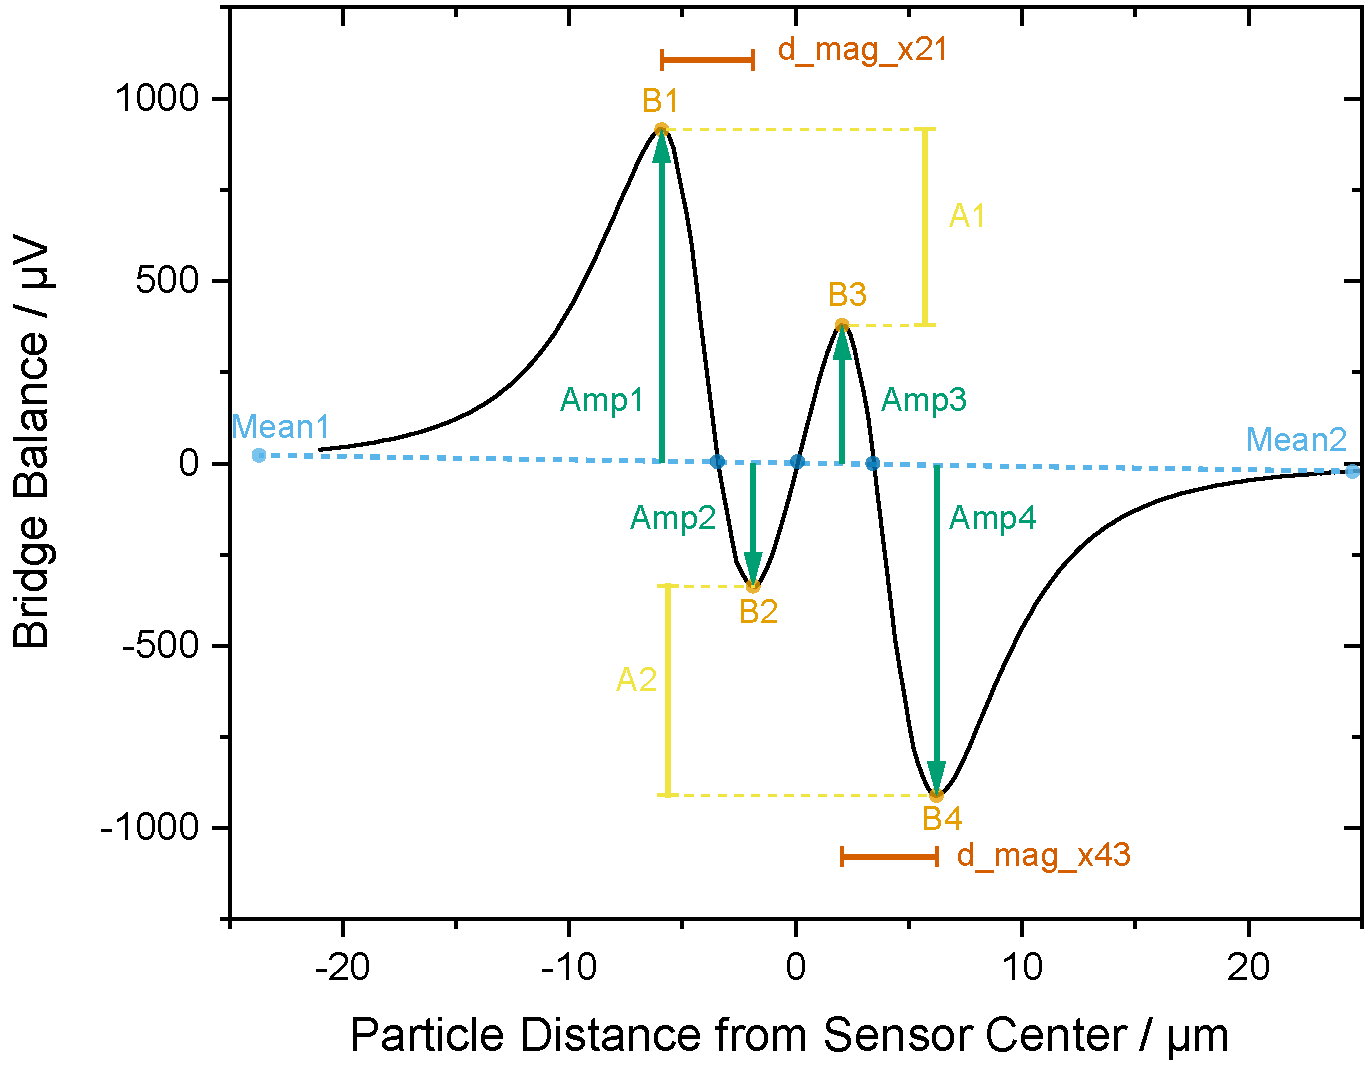
\includegraphics[width=.7\linewidth]{Ressources/Simulation/ExampleSignal}
	\capption{Example Signal of Magnetic Measurement}{Signals generated from the Wheatstone bridge sensor setup feature a certain shape which allows for several measures. In case the overall signal stream carries a constant or linear offset, it is scaled to the means before and after the detected peak pattern. (\textcolor{OlightBlue}{Mean1, Mean2}) The x- and y-positions of each peak are denominated by \textcolor{Oorange}{B1-4} and \textcolor{Ogreen}{Amp1-4}, respectively. The crossings of the signal through the linear connection of both means are denominated by \textcolor{OdarkBlue}{n1-3} (in the figure by \darkBlueCircle). Further, the difference between the equally oriented peaks \textcolor{Oorange}{B3}-\textcolor{Oorange}{B1} and \textcolor{Oorange}{B4}-\textcolor{Oorange}{B2} gives a measure for the homogeneous movement of the measured object and are called \textcolor{Oyellow}{A1} and \textcolor{Oyellow}{A2} each. From these values, the overall velocity $v$ can be approximated because the \gls{dgmr} and \gls{fs} are fixed precisely. Analogously, the magnetic diameter of a dipole is computed by the mean of the differences \textcolor{Oorange}{B2}-\textcolor{Oorange}{B1} and \textcolor{Oorange}{B4}-\textcolor{Oorange}{B3}.}
	\label{fig:conc:example}
\end{figure}

By measuring the absolute concentration with a commercially available flow cytometer (MacsQuant 10, Miltenyi), a reference bead count was established. In a pre-test, beads were taken directly from the microcentrifuge tube, after pumping through a syringe, and after pumping through a syringe with \SI{10}{\centi\meter} of connected through tubing (ID \SI{0.5}{\milli\meter}, RS Chemicals). Afterward, they were counted in the flow cytometer in equal volumes. Additionally, two different buffers - \gls{macs} and \gls{pbs} - and two different surface terminations were used. Both buffers are based on \acrfull{pbs}. Notwithstanding \gls{macs} contains \gls{edta} as a chelator for divalent ions, Tween 20\footnote{a non-ionic surfactant}, and an azide-based stabilizer. Hence, the wetting of surfaces and the electrostatic interactions of these buffers differ. The same properties were varied on the bead surface by choosing acrylate- and biotin-terminated beads.\\
In \cref{fig:conc:losses_syringe}, a trend (without statistical confidence) can be observed that shows a decrease in particle counts after every additional surface with which beads could potentially interact. In term, a correct count in absolute numbers seems out of range. However, a calibration of the system with the flow profile inside the channel to compensate for losses subjected to connectors and magnetic enrichment structures was carried out successfully.
\begin{figure}[b]
	\centering
	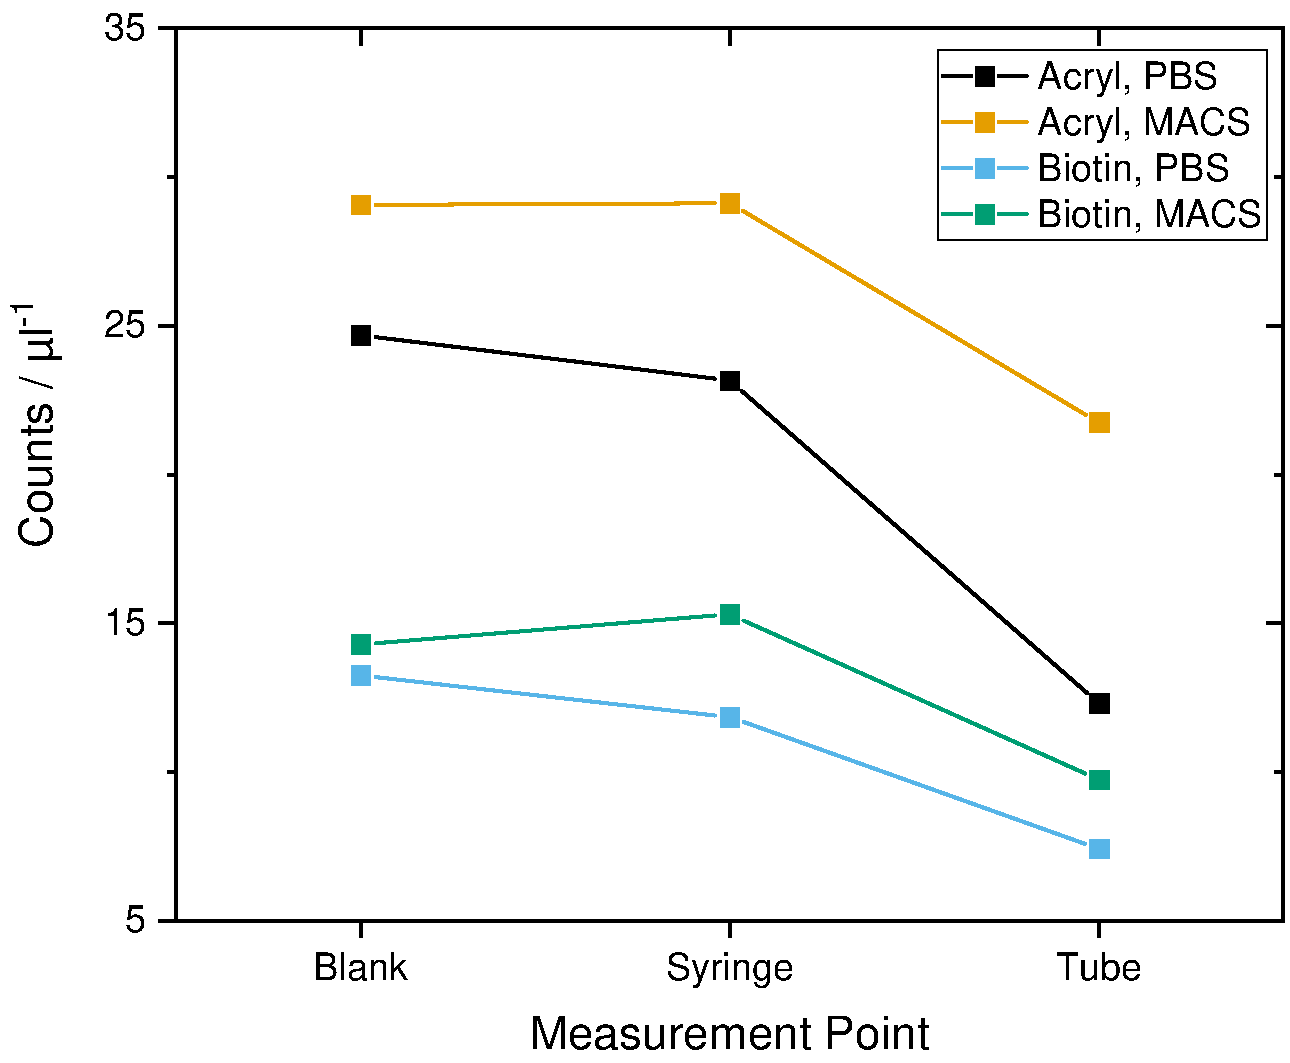
\includegraphics[width=.7\linewidth]{Ressources/Concentration/Losses-Syringe-Tubing}
	\capption{Bead Loss Evaluation in Connectors}{Bead concentrations measured in equal volumes in the flow cytometer after being pumped through a syringe or a syringe with connected tubing. The blank sample was measured directly from the stock solution. Additionally, electrostatic and surface-tension related effects were resolved by the usage of different buffers and bead surfaces.}
	\label{fig:conc:losses_syringe}
\end{figure}


\clearpage
\subsection{Measurement Error Sources and Calibration of Flow Field}
\label{sec:res:Correction}
In order to account for the bead losses due to the tubing connectors, the Hagen-Poiseuille flow profile, and magnetophoretic enrichment structures, the measured bead concentration was corrected in two different approaches.(\cref{eq:corr:conc}) On the one hand, the typical assay correction to the ground truth by a constant \gls{corrConst} computed from the blank population was established. On the other hand, a \gls{corrVel} compared the \acrfull{umean} to the \gls{vc}.
\begin{equation}	
	c_\text{beads,\, expected} = c_\text{beads,\, measured}  \cdot C \label{eq:corr:conc}
\end{equation}
The \gls{corrConst} relates a reference count in the optical flow cytometer to the measurement in the magnetic flow cytometer.(\cref{eq:corr:const}) Equally-adjusted bead concentrations in the samples allow for a correction to the reference system. However, for an assay usage, the initial concentration of beads either has to be known precisely or has to be irrelevant, for example in regards to a standardized measurement procedure. Besides, \gls{corrConst} provides a reliable and generalizable option for correction. 
\begin{align}
	C_\text{const} &= \frac{c_\text{beads, standard procedure}}{c_\text{beads, MRCyte}} \label{eq:corr:const}\\
	v_\text{c} &= 2\ d_\text{gmr} \frac{f_\text{s}}{n_\text{3}-n_\text{1}} \label{eq:v:c} \\
	C_\text{velocity} &= \frac{\overline{\mathbf{u}}}{v_\text{c}} = \frac{Q}{A \cdot v_\text{c}} \label{eq:corr:vel} 
\end{align}
The \gls{corrVel} relates the effective particle velocity to the total fluid velocity in order to eradicate flow profile provoked effects.(\cref{eq:corr:vel}) Whereas \gls{umean} was determined by \acrfull{q} through a cross-sectional \gls{a} of the channel, \gls{vc} was analyzed from the measured signal stream. Here, the intrinsic \acrfull{dgmr} was divided by the time difference where the bead passed exactly over a half-bridge with known distance.(\cref{eq:v:c}) These specific timepoints are visible as dimensionless zero-crossings $n_\text{1}$ and $n_\text{3}$ in the signal and can be converted by scaling with the \acrfull{fs} into the time domain.(\cref{fig:conc:example})
\clearpage
\begin{figure}[h!]
	\centering
	\subfloat{
		\subfigimg[height=150pt]{a}{Ressources/Concentration/BiotinylWrongCorrection}
		\phantomsubcaption
		\label{fig:conc:BiotnylWrongCorr:velConst}	
	} \hfill
	\addtocounter{subfigure}{-1}
	\subfloat{
		\subfigimg[height=150pt]{b}{Ressources/Concentration/BiotinylTime}	
		\phantomsubcaption
		\label{fig:conc:BiotnylWrongCorr:time}
	}
	\capption{Error Sources in Concentration Measurements}{(\textbf{a}) Robustness evaluation of both correction factors \gls{corrConst} and \gls{corrVel} for protein-coated surfaces. The mean and \gls{sem} of plain and biotinylated measurements show a high deviation from physically reasonable expectations when corrected for the velocity (right). In contrast, \gls{corrConst} can intrinsically correct only well below \SI{100}{\percent}. (\textbf{b}) Mean and \gls{sem} of a fit-corrected bead capture experiment with several error sources. Initially, the magnetophoretic structures have to be filled and thus decrease the plain count for the first \SI{100}{\micro\liter}. (\orangeline) Additionally, the high deviation offsets the correction factor so that the stable measurement from \SIrange{100}{200}{\micro\liter} lies now above the ideal reference. In contrast, the biotinylated beads are captures by the surface functionalization and hence a very low concentration is measured. However, a steep rise with pulsations can be observed when the surface is saturated with beads and the particles begin to flow over the sensor in bursts. (\blueline) The abrupt decline to the end of the measured volume is most probably related to sedimentation effects inside the emptying syringe.}
	\label{fig:conc:BiotnylWrongCorr}
\end{figure}
\begin{figure}[h!]
	\centering
	\subfloat{
		\subfigimg[height=150pt]{a}{Ressources/Concentration/ConcentrationError}	
		\phantomsubcaption
		\label{fig:conc:AbsConcError:concerror}
	} \hfill
	\addtocounter{subfigure}{-1}
	\subfloat{
		\subfigimg[height=150pt]{b}{Ressources/Concentration/ConcentrationVelocity}	
		\phantomsubcaption
		\label{fig:conc:AbsConcError:vel}
	}
	\capption{Absolute Concentration Measurements}{(\textbf{a}) Mean and standard deviation of the concentration measurement from three independent measurements. The uncorrected measurement shows a highly reproducible and linear count over the dynamic range of almost two decades. (\greenrect) The ideal reference from the flow cytometer is depicted in (\blackline). Correction with \gls{corrVel} (\orangerect) yields at a factor of \num{2,26109} which is \SI{21.7}{\percent} more imprecise than \gls{corrConst} at \num{2,88833 +- 0,08075}.(\bluerect) (\textbf{b}) Mean and \gls{sem} of the \gls{vc} estimation from the signal. For higher concentrations, the measured velocity becomes inaccurate thus distorts the correction factor.}
	\label{fig:conc:AbsConcError}
\end{figure}
\clearpage
However, if the bead velocity is not solely dependent on fluid dynamic effects - especially in the light of surface functionalizations - \gls{corrVel} can not be applied to experiments robustly. This is depicted in a sample experiment with a protein-covered surface in \cref{fig:conc:AbsConcError:concerror}. By definition, the \gls{corrConst} can not be well above \SI{100}{\percent} whereas the count correction by \gls{corrVel} differs by \SI{600}{\percent} through variations in the velocity measurement.(\cref{fig:conc:BiotnylWrongCorr:velConst})

An adaptation of these corrections to real measurements is depicted in \cref{fig:conc:AbsConcError}. In a measurement where \SI{300}{\micro\liter} were dispensed into the magnetic flow cytometer with a defined particle concentration, the counts were analyzed and corrected according to above. This time, the channel had a cross-section of \SI{700}{\micro\meter} $\times$ \SI{50}{\micro\meter} (\gls{chanW} $\times$ \gls{chanH}) and \gls{q} was set to \SI{30}{\micro\liter\per\minute}.\\
Apart from a reproducible count over the dynamic range of almost two decades, both correction factors ameliorated the present data. \gls{corrConst} amounted in an optimum of \linebreak \num{2,89 +- 0,08} while \gls{corrVel} centered around a mean of \num{2,26}. Consequently, the velocity correction was misguided by \SI{21.7}{\percent} for the advantage of requiring no \textit{a priori} knowledge about the measurement.\\
Another peculiarity of \gls{corrVel} can be observed in \cref{fig:conc:AbsConcError:vel}. While the analyzed velocity is stable for less than \SI{10}{\per\micro\liter}, a linear decrease is visible for higher concentrations. This is a consequence when signals of beads start overlapping if these are flowing over the sensor in close vicinity. Hence, the disturbed signal sensitizes the parameter reconstruction to errors such as false peak identification.
\clearpage
\subsection{Concentration Measurement in Diluted Whole Blood}
\label{sec:res:wholeBlood}
The same concentration measurements from before were now carried out in whole blood samples. Here, the reference count can be attained only below the experimentally determined critical concentration of approximately \SI{10}{\per\micro\liter}. (\cref{fig:conc:blood}) An insignificant discrepancy could be perceived in different volumetric blood to buffer dilutions of 1:1 and 1:20, respectively. This provides evidence for the measurement's independence from the blood concentration in a buffer. \\
However, a significant difference between counts was discovered between a \SI{150}{\micro\meter} high channel, where \gls{corrVel} can be determined accurately, and a \SI{50}{\micro\meter} high channel, where the correction yields a great error to the reference. This may be subjected to an increased probability of collisions from beads with blood cells and hence a decreased velocity which in turn leads to a higher correction factor. Another explanation approach could be the transition from \textit{Newtonian} to \textit{Non-Newtonian} fluid dynamics in smaller cross-sections, which could likewise be influenced by the F\aa{}r\ae{}us effects mentioned in \cref{sec:theo:faraeus}.
\begin{figure}[h!]
	\centering
	%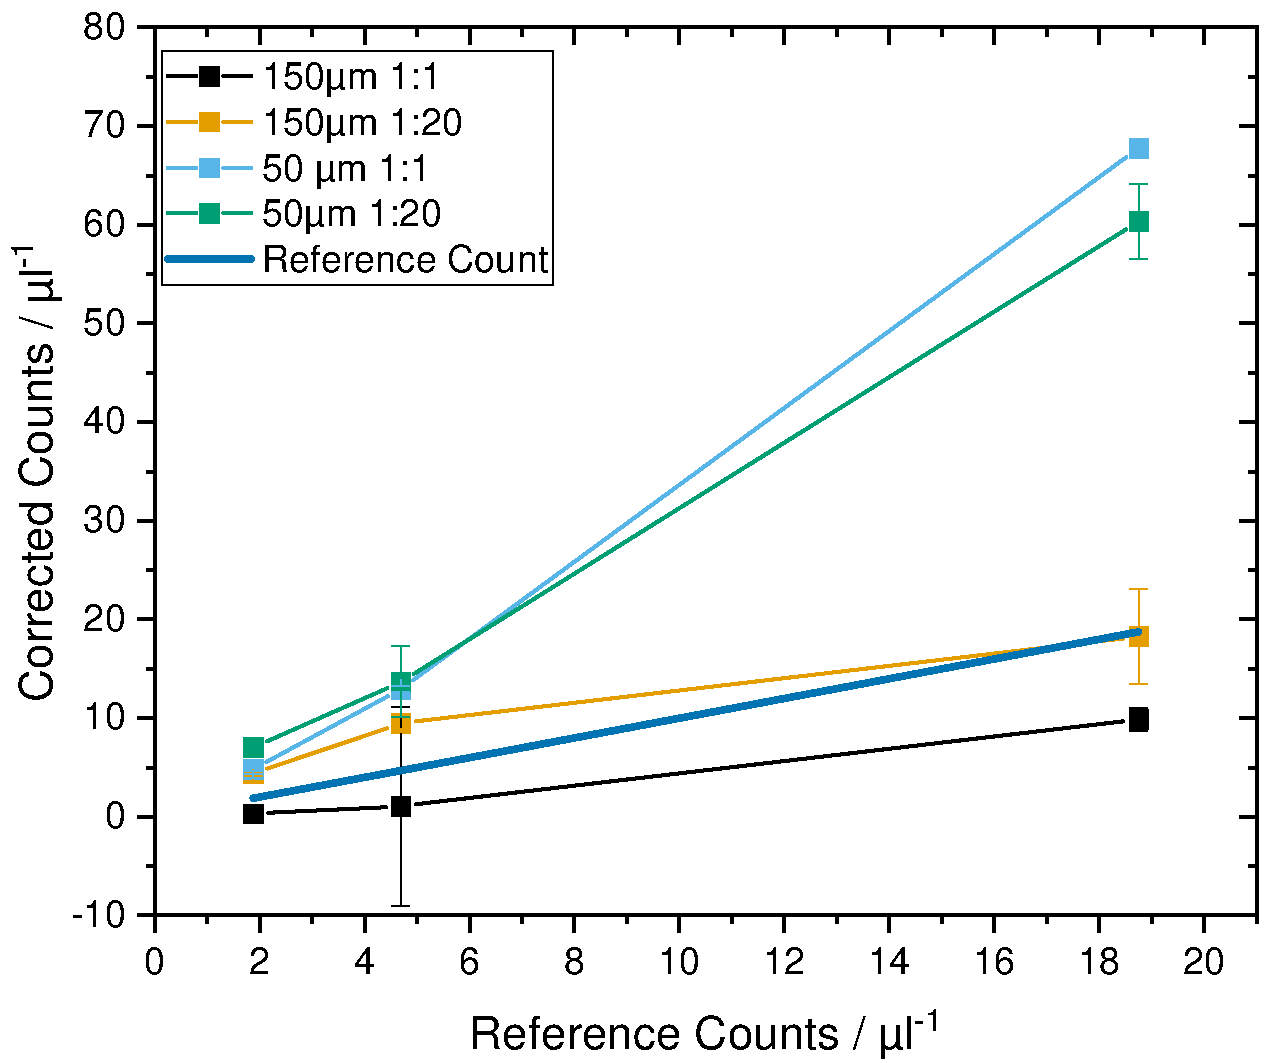
\includegraphics[width=.7\linewidth]{Ressources/Concentration/CorrectionBlood}
	\subfloat{
		\subfigimg[height=150pt]{a}{Ressources/Concentration/Correction_50um}	
		\phantomsubcaption
		\label{fig:conc:blood:50}
	} \hfill
	\addtocounter{subfigure}{-1}
	\subfloat{
		\subfigimg[height=150pt]{b}{Ressources/Concentration/Correction150um}	
		\phantomsubcaption
		\label{fig:conc:blood:150}
	}
	\capption{Absolute Concentration Measurement in Blood Samples}{Velocity corrected concentration measurements for two different blood dilutions and channel heights. While \gls{corrVel} shows a good approximation for high channels in all tested concentrations (\textbf{a}), it does exaggerate the data for high concentrations at \gls{chanH}= \SI{50}{\micro\meter}.(\textbf{b}) This is probably a result of bead-cell collisions and the resulting path interruptions. }
	\label{fig:conc:blood}
\end{figure}
\clearpage
\subsection{Differential Counting Setup}
\label{sec:res:diffCounting}
With regard to the necessity of correction factors, a different magnetic flow cytometer setup has been evaluated to resolve the ground truth of a concentration measurement. Here, two fully assembled sensors with \glspl{pcb} were stacked on top of each other and connected in series which was expected to yield two beneficial effects.\\
First, one permanent magnet underneath the lower sensor chip should supply both chips with enough gradient field to pull beads to the respective channel bottom. Second, the simultaneous signal acquisition should act on the one side as a time-of-flight detector with a relatively long transport distance and on the other side, a differential concentration measurement was envisioned between both chips. Therefor, the hypothetical optimum parameter set could be reached when the relative concentration measurement yielded identity:
\begin{equation}
	\dfrac{c_\text{\ top sensor}}{c_\text{\ bottom\ sensor}} \overset{!}{=} 1
	\label{eq:diff:optimum}
\end{equation}
The system comprises two separately assembled sensor \glspl{pcb} with nylon spacers between the positional screws.(\cref{fig:diff:sensitivity})  A \SI{3}{\milli\meter} hole was drilled into the top \gls{pcb} carefully between the strip lines to minimize the tubing length from the top chip outlet to the bottom chip inlet. 
After the build-up of the differential counting system,\footnote{as described in \cref{sec:meth:dualGMR}} the hysteresis of both sensor elements was maximized for sensitivity and the concentration was measured against a reference from the optical flow cytometer. 
\begin{figure}[h!]
	\centering
	\subfloat{
		\subfigimg[width=\linewidth]{a}{Ressources/Differential/setupSide}	
		\phantomsubcaption
		\label{fig:diff:sensitivity:setupSide}
	}\\
	\vspace{\baselineskip}
	\addtocounter{subfigure}{-1}	
	\subfloat{
		\subfigimg[height=150pt]{f}{Ressources/Differential/Optupper}	
		\phantomsubcaption
		\label{fig:diff:sensitivity:optTop}	
	} \hfill
	\addtocounter{subfigure}{-1}	
	\subfloat{
		\subfigimg[height=150pt]{g}{Ressources/Differential/Optlower}	
		\phantomsubcaption
		\label{fig:diff:sensitivity:optBottom}	
	}
	\capption{Hysteresis Calibration for Stacked \Gls{pcb} Setup}{(\textbf{a}) Differential measurement setup: the system comprises two separately assembled sensor \glspl{pcb} (\textbf{b}) with nylon spacers (\textbf{e}) between the positional screws. (\textbf{f}) A hole with a \SI{3}{\milli\meter} diameter was drilled between the strip lines to connect the top chip outlet to the bottom chip inlet and minimize tubing length thereby. Schematically, a permanent magnet is placed below the bottom \gls{pcb}.(\textbf{d})  The field line density respectively the area with negligibly differing field vectors are shown in the blue triangle. Because the adjustment is always carried out for a single bridge at once, this causes a systematic error.\\
		The magneto-resistive effects of both sensors, calculated from their hystereses, are depicted for top and bottom sensors, respectively. Whereas the hysteresis was optimized for the centered sensor bridge (D or E) on the top sensor in (\textbf{f}), it was  optimized for the bottom sensor in (\textbf{g}). Additionally, the height of the nylon spacers was varied from \SIrange{3}{8}{\milli\meter} but showed no statistical correlation.}
	\label{fig:diff:sensitivity}
\end{figure}
\clearpage
\subsubsection{Sensitivity Calibration}
Initially, the permanent magnet was adjusted in three linear directions in order to maximize the magnetic sensitivity of both Wheatstone bridges. Schematically, this can be envisioned as placement of the whole top as well as the whole bottom bridge configuration into the operational range of the magnet, which is indicated by the blue triangle.

Then, the hysteresis of both outermost and one centered sensor was optimized for their full coverage and sensitivity. The recorded values for a sole optimization of the top or bottom sensor array with a height variation of the utilized nylon spacers are shown in \cref{fig:diff:sensitivity:optTop,fig:diff:sensitivity:optBottom}. The optimized sensor exhibits a monotonously higher \gls{mr} than the disregarded bridge. Nevertheless, the complete sensor setup features an \gls{mr} well above \SI{7.2}{\percent} which is acceptable both for measuring immunomagnetically labeled cells and magnetic microbeads. Furthermore, the homogeneity of the interspersing magnetic field can be monitored in the triangular shape of every acquired curve in the sensitivity plots. As the field vectors of \gls{B} start to disperse at the outsides of the illustrated blue area in \cref{fig:diff:sensitivity}c, the outer sensor regions are not located completely inside a homogeneous gradient field and get distracted by non-perpendicular field components.\citet{lit:thes:helou} \\
Additionally, no influence of any spacer height could be discovered.  The difference in \gls{mr} varied insignificantly in \SI{0.14 +- 0.6}{\percent} of \gls{mr}.
\clearpage


\subsubsection{Magnetic Concentration Measurement with the Differential Sensor Setup}
Due to the single utilized permanent magnet for two sensors, another field-related issue arose during concentration measurements. This requires a step back inside the general functionality of the magnetophoretic enrichment:\\
Any bead flowing at an arbitrary position in the microchannel experiences a negative magnetic force by the gradient of the \acrlong{B} caused by the permanent magnet which pulls perpendicular to the bottom surface. Upon coming near the lower boundary, a gradient provoked by the lithographic nickel-iron structures starts to gain strength with the third power of the distance. This causes the beads to attach to the bottom firmly and enforces their rolling behavior. However, a fragile equilibrium between magnetophoresis and drag has to be maintained slightly in favor of \acrlong{f:drag} for a continuous rolling motion.

This ideal state is a narrow space in between two boundary cases:\\
First, if drag force exceeds magnetophoresis, the beads will not migrate to the channel bottom in the top chip and hence result in a lower concentration measured on top. Second, if magnetophoresis outnumbers drag so that particles flow steadily in the top channel, the beads in the lower channel will stop rolling and adhere. In effect, the lower concentration measurement is compromised. This behavior is visible in \cref{fig:diff:sensitivity:top,fig:diff:sensitivity:bottom}.\\
In order to find the flow rate for the optimal ratio between drag and magnetic force, measurements were performed with bead concentrations ranging from \SIrange{8.5}{34}{\per\micro\liter}. The respective quotient was determined after \cref{eq:diff:optimum} and plotted in \cref{fig:diff:optimum}. Below an optimal threshold of \SI{160+-10}{\micro\liter\per\minute}, the top sensor measures up to the 100-fold concentration of the bottom sensor. Above the threshold, the top sensor starts to miss counts which is subjected to a high drag force relative to the magnetophoresis. The quotient of both sensors shows a linearly decreasing trend towards saturation at high flow rates where no beads are measured by both sensors.\\
Hereby, the intersection of all measured concentrations does not reside in \num{1}, at the optimal value of the quotient. This can on the one side be attributed to the numerical velocity correction and on the other side to the losses in the interconnection between both chips. Although the optimal quotient value would have been \num{1} theoretically, an ideal overlap was found for a flow rate of \SI{150}{\micro\liter\per\minute}.

The determined optimal flow rate prohibits a functionalization inside the respective channel due to the high shear forces of \SI{11.8}{\dyne\per\centi\meter}. Therefore, a bio-functionalized channel has to be designed with a greater hydrodynamic diameter to lower velocity and shear. Therefore, two channels have been designed and probed initially. First, a simple serpentine channel with a width of \SI{1}{\milli\meter} has been developed to bond onto an assembled sensor.(\cref{fig:app:serpentine}) Second, in another approach, a focusing structure with an aperture of \SI{30}{\micro\meter} width for the sensor element itself has been designed.(\cref{fig:app:focus}) However, the difficulties in assembly and operation of the whole setup inhibited its usage in further experiments.

\begin{figure}[h!]
	\centering
	\begin{minipage}[b]{.3\linewidth}
			\subfloat{
			\subfigimg[width=\linewidth]{a}{Ressources/Differential/Top}	
			\phantomsubcaption
			\label{fig:diff:sensitivity:top}
		}\\
		\vspace{-8pt}
		\addtocounter{subfigure}{-1}	
		\subfloat{
			\subfigimg[width=\linewidth]{b}{Ressources/Differential/Bottom}	
			\phantomsubcaption
			\label{fig:diff:sensitivity:bottom}	
		}
	\end{minipage}%
	\hfill
	\begin{minipage}[b]{.68\linewidth}
		\addtocounter{subfigure}{-1}	
		\subfloat{
			\subfigimg[width=\linewidth]{c}{Ressources/Differential/Differential}	
			\phantomsubcaption
			\label{fig:diff:sensitivity:quot}	
		}
	\end{minipage}
%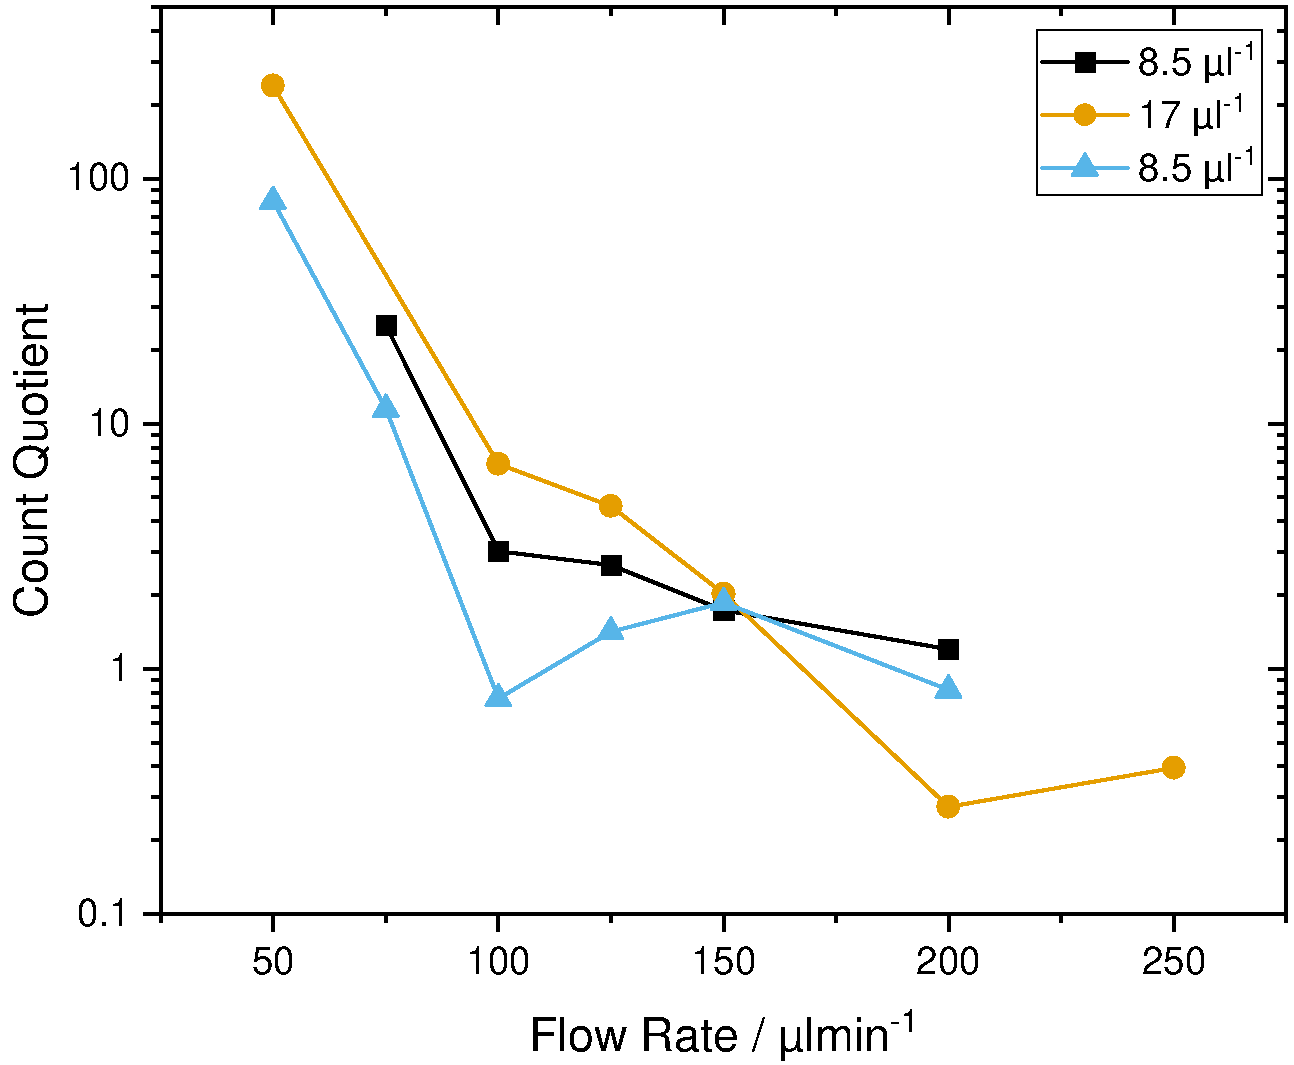
\includegraphics[width=]{Ressources/Differential/Differential}
	\capption{Optimal Differential Counting Flow Rate}{The optimal flow rate for the differential setup was determined by the quotient of measured concentrations between the top (\textbf{a}) and bottom (\textbf{b}) sensor.(\textbf{c}) Below an optimal threshold of \SI{150}{\micro\liter\per\minute}, the top sensor measures up to the 100-fold concentration of the bottom sensor. Above a threshold, the top sensor starts to miss counts which is subjected to the high drag force. (\textbf{c}) The quotient of both sensors $\frac{\text{top}}{\text{bottom}}$ shows a linearly decreasing trend towards a saturation at high flow rates where no beads a measured at both sensors. Hereby, the intersection of all measured concentrations does not reside in \num{1}, at the optimal value of the quotient. This can on the one side be attributed to the \acrlong{corrVel} and on the other side to the losses in the interconnection between both chips.}
	\label{fig:diff:optimum}
\end{figure}
\clearpage
\subsection{Surface Magnetization of Biofunctionalized Beads}
\label{sec:res:beadMangetiz}
Here, the previously surface-modified polystyrene beads were magnetized with \glspl{mnp} and counted in the magnetic flow cytometer. Originally, four different \acrlongpl{mnp} have been tested. Albeit, both nanomag-D-spio \SI{100}{\nano\meter} (micromod Partikeltechnologie GmbH, Rostock) and dynabeads MyOne Streptavidin C1 \SI{1}{\micro\meter} (ThermoFisher scientific, Waltham, USA) showed inconclusive results and are omitted in the latter.

First, BNF-Dextran-redF-streptavidin \SI{100}{\nano\meter} \glspl{mnp} (micromod Partikeltechnologie GmbH, Rostock) were attached to the non-magnetic beads after the protocol in \cref{sec:meth:coatingMNPs}. Then, the magnetizability was examined qualitatively in a magnet stand. Particles were considered ``magnetically labeled'' if a pellet was visible after \SI{10}{\minute}. Afterward, the concentrations were measured with the optical flow cytometer and adjusted to \SI{10 +- 1}{\per\micro\liter} accordingly.

The subsequent measurement of \SI{300}{\micro\liter} in the magnetic flow cytometer is shown in \cref{fig:conc}. In \cref{fig:conc:BNF:c1} the peak difference C1 (= Amp2 - Amp1, \cref{fig:conc:example}) is presented against the biotinylation degree. Independent experiments of \SIlist{100;68}{\percent} biotinylation show a certain amplitude difference. The respective fluid and particle velocities in \cref{fig:conc:BNF:vc} provide an explanation for this behavior. The fluid velocity had to be adapted during the course of the experiments from \SIrange{80}{10}{\micro\liter\per\minute} to receive stable counts.\\
Keeping this in mind leads to the fact that - although only two biotinylation coverages were measured - four distinct magnetizations are represented here. Both \SI{100}{\percent} samples show slow but plausible velocities and can therefore be correlated with differing magnetic moment. Beads with \SI{68}{\percent} show an exceptional velocity and can hence either be considered as noisy background or very weakly magnetized particles that are not pulled to the channel bottom completely. This could also explain the decline in C1 which is also a measure for \acrlong{m}.

%\begin{figure}[h!]
%	\centering
%	\subfloat{
%		\subfigimg[height=150pt]{a}{Ressources/Concentration/OceanC1}
%		\phantomsubcaption
%		\label{fig:conc:Ocean:C}	
%	} \hfill
%	\addtocounter{subfigure}{-1}
%	\subfloat{
%		\subfigimg[height=150pt]{b}{Ressources/Concentration/OceanVc}
%		\phantomsubcaption
%		\label{fig:conc:Ocean:vc}	
%	}
%	\capption{Bead Coverage Assay with OceanNanotec \SI{50}{\nano\meter}}{Magnetic flow cytometry data from \SI{8}{\micro\meter} polystyrene sphere which were biotinylated in different degrees and subsequently coated with SV0050 \SI{50}{\nano\meter} streptavidin \glspl{mnp} (OceanNanotech, San Diego, USA). Mean from 3 different particle distributions at maximum coverage(\textbf{a}) d = \SI{4}{\micro\meter} (\textbf{b}) d = \SI{8}{\micro\meter}}
%	\label{fig:conc:Ocean}
%\end{figure}
\clearpage
Second, SV0050 \SI{50}{\nano\meter} streptavidin \glspl{mnp} (OceanNanotech, San Diego, USA) were deposited after the equal procedure on \SI{8}{\micro\meter} polystyrene beads. These experiments show the expected result of declining peak amplitude at lower biotinylation and constant velocity throughout. (\cref{fig:conc:Ocean:C,fig:conc:Ocean:vc}) At a p-value smaller than \SI{10}{\percent}, the high populations differ significantly from each other while the log-normal fits match the histograms with a \gls{rsquadj} of \num{0.94}.\\
Two hypotheses can be drawn now from this result. On the one side, OceanNanotech \glspl{mnp} could possess more magnetic moment per particle, which favors the robust measurement. On the other side, streptavidin or \gls{mnp} size could influence the saturation of all available biotin sites of the particle. 

\begin{figure}[h!]
	\centering
	\subfloat{
		\subfigimg[height=150pt]{a}{Ressources/Concentration/BNFC1}
		\phantomsubcaption
		\label{fig:conc:BNF:c1}	
	} \hfill
	\addtocounter{subfigure}{-1}
	\subfloat{
		\subfigimg[height=150pt]{b}{Ressources/Concentration/BNFVc}	
		\phantomsubcaption
		\label{fig:conc:BNF:vc}
	} \\
	\vspace{\baselineskip}
	\subfloat{
		\subfigimg[height=150pt]{c}{Ressources/Concentration/OceanC1}
		\phantomsubcaption
		\label{fig:conc:Ocean:C}	
	} \hfill
	\addtocounter{subfigure}{-1}
	\subfloat{
		\subfigimg[height=150pt]{d}{Ressources/Concentration/OceanVc}
		\phantomsubcaption
		\label{fig:conc:Ocean:vc}	
	}
	\capption{Bead Coverage Assay with Magnetic Streptavidin Nanoparticles}{Magnetic flow cytometry data from \SI{8}{\micro\meter} polystyrene sphere which were biotinylated in different degrees and subsequently coated with BNF-Dextran-redF-streptavidin \SI{100}{\nano\meter} \glspl{mnp}(\textbf{a},\textbf{b}) or SV0050 \SI{50}{\nano\meter} streptavidin \glspl{mnp} (\textbf{c},\textbf{d}). (\textbf{a}) Signal amplitude of the counts with various flow rates  1. \SI{80}{\micro\liter\per\minute} 2. \SI{40}{\micro\liter\per\minute} 3. \SI{20}{\micro\liter\per\minute} 4. \SI{10}{\micro\liter\per\minute} (\textbf{b}) Reconstructed velocities of the respective populations. The \SI{100}{\percent} biotinylation shows plausible velocities, whereas the \SI{68}{\percent} sample can either be considered as noisy background or very weakly magnetized particles.(\textbf{c}) Signal amplitude with \SI{80}{\micro\liter\per\minute}. A correlation between biotinylation degree and magnetic moment can be assumed at a p-value p < \num{0.1} (\textbf{d}) Velocity distributions of the samples. As postulated, the mean velocities do not differ, moreover, are enveloped by the blank sample.}
	\label{fig:conc}
\end{figure}


\clearpage
\section{Surface Modification and Biofunctionalization of the Sensor Chip Substrate}
\label{sec:res:surfMod}
In consideration of the problems of surface instability, analyzed in \cref{sec:res:Correction}, and to avoid additional uncertainties in the experimental validation of the model from \cref{sec:res:forcesim}, covalent functionalizations of the sensor surface with neutravidin were carried out. First, a plate reader experiment for a qualitative statement about the shear-force stability of protein adsorption was performed. Second, different functionalization approaches with \gls{piranha} and \gls{hf} were tested with pure glass, \gls{pdms}, and eventually \gls{sin}. Third, the validation of these procedures was limited to indirect measurements such as tensiometry, fluorescence microscopy, and quantitative bead capture assay, as sophisticated chemical analyses were hardly available.

\subsection{Physisorption}
\label{sec:res:physis}
In order to quantify the adsorption stability for fluorescently-labeled, physisorbed streptavidin molecules, sensor chips were cut into \SI{10}{\milli\meter\squared} pieces and glued to the bottom of a 96-well plate. Subsequently, they were equilibrated with \gls{pbs} and incubated with \SI{1}{\milli\gram\per\milli\liter} overnight. Each measurement was corrected for a blank substrate as well as the negative control with plain \gls{pbs} buffer and normalized subsequently.

\begin{figure}[h!]
	\centering
	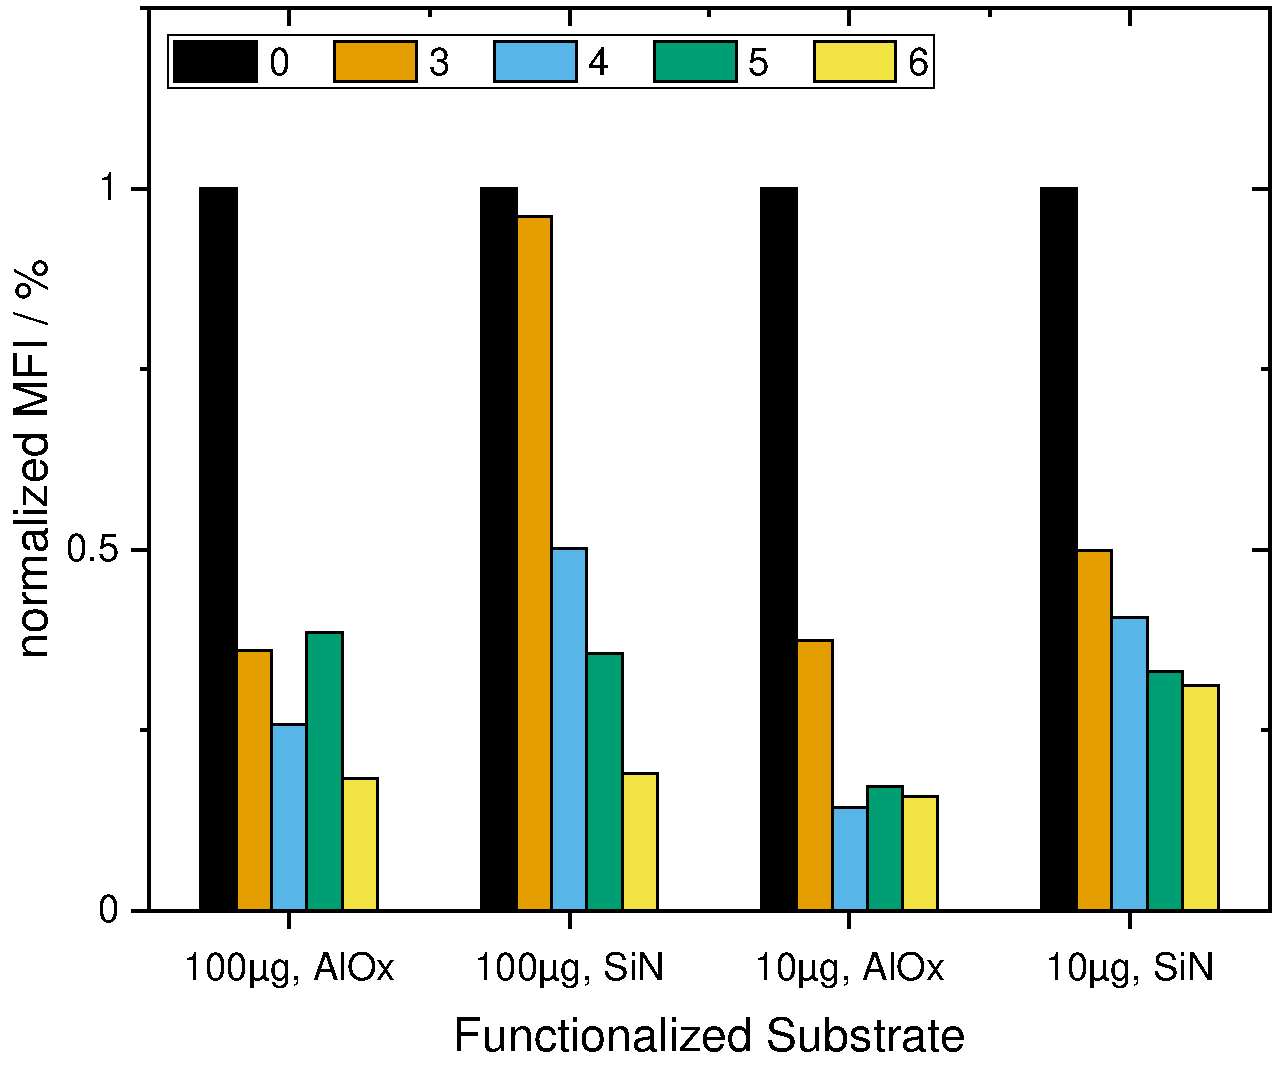
\includegraphics[width=.7\linewidth]{Ressources/ResultPlots/SurfaceFuncSiNAlOx}
	\capption{Surface Adsorption Stability of Neutravidin on \Gls{sin} and \Gls{alox}}{Plate reader measurement with \SI{3}{\milli\meter} $\times$ \SI{3}{\milli\meter} \gls{sin} and \gls{alox} samples which were incubated with \SI{100}{\micro\gram} and \SI{10}{\micro\gram} streptavidin-atto488, respectively. The samples were subsequently washed with \SI{200}{\micro\liter} \gls{pbs} carefully. Fluorescence intensities were corrected with a blank substrate, the autofluorescence of \gls{pbs}, and normalized eventually. Every surface reaches a mean fluorescence level of \SI{28}{\percent} after few washing steps.}
	\label{fig:unsp:wash}
\end{figure}
Every sample in the plate reader showed a significant surface decrease to a mean level of \SI{28}{\percent} from the original fluorescence.(\cref{fig:unsp:wash}) Whereas proteins desorbed from both crystals after the first washing steps equally, \gls{sin} outperformed \gls{alox} as more stable in a steady state. (\SI{34.8}{\percent} vs. \SI{27.5}{\percent}) However, no quantitative hypothesis could be formulated by these numbers due to the nature of their indirect measurement. Hence, the protein activity which is the crucial quantity for any bead rolling remains questionable. Nevertheless, a qualitative proposition is strongly confirmed that unspecifically adsorbed proteins are removed from any of both surfaces rapidly.

\clearcaptionsetup{float type}
\subsection{Evaluation of the Covalent Biofunctionalization with Optical Methods}
\label{sec:res:coval}
Now, the results of several covalent surface modification procedures with various substrates are presented. Foremost, glass was used as the main carrier material. On glass established protocols were then brought onto \gls{pdms} and \gls{sin} chips. As the main functionalization protocol, an activation in 7:1 \gls{piranha} was carried out for \SI{30}{\minute}. Then, the substrate was rinsed, incubated in \SI{2}{\percent} \gls{aptes} solution and in \gls{paa} subsequently after the protocol described in \cref{sec:meth:surfFunc}. Then a \SI{150}{\micro\meter} microfluidic channel was glued to the functionalized substrate and eventually filled with \SI{1}{\milli\gram\per\milli\liter} of neutravidin or streptavidin-atto488 if fluorescent labeling was intended. A constant flow rate of \SI{80}{\micro\liter\per\minute} was selected for the bead capture assays under the light microscope. The general process chain is depicted in \cref{fig:chem:func:withPAA}.


As a final result, a chemical and biological functionalization could be established to a similar degree as unspecific binding. Measuring the count of beads per occupied area yields \cref{fig:coval:densitysubstrate}. Again, two distinct states can be observed for biotinylated and plain beads at every modified surface.\\
The density of bound protein could also be varied through the incubation concentration and measured reliably both in an optical bead capture assay and the \gls{mfi} of the channel in a fluorescence microscope.(\cref{fig:coval:counts,fig:coval:titration}) The relative \gls{mfi} indicates here the fraction supra the non-functionalized, \gls{pbs}-filled microchannel. 

However, a substantially different long-term stability could neither be measured nor compared to similar results accurately. Also, no proof for the covalent functionalization could be brought with the available methods. Nevertheless, a robust and working protocol has been developed after significant literature values which encourages the position.
\begin{figure}[htb!]
	\centering
	\begin{minipage}[b]{.3\linewidth}
	\subfloat{
		\subfigimg[height=95pt]{a}{Ressources/Covalent/PositivePiranhaPAA}
		\phantomsubcaption
		\label{fig:coval:biotinyl}		
	} \\ 
	\vfill	
	\addtocounter{subfigure}{-1}
	\subfloat{
		\subfigimg[height=95pt]{b}{Ressources/Covalent/NegPiranhaPAA}
		\phantomsubcaption
		\label{fig:coval:plain}		
	}
	\end{minipage}%
	\hfill
	\begin{minipage}[b]{.7\linewidth}
	\addtocounter{subfigure}{-1}
	\subfloat{
		\subfigimg[width=\linewidth]{c}{Ressources/Covalent/BeadDensitySubstrate}
		\phantomsubcaption
		\label{fig:coval:densitysubstrate}		
	}
	\end{minipage}% 
	\\
	\vspace{\baselineskip}
	\addtocounter{subfigure}{-1}
	\subfloat{
		\subfigimg[height=150pt]{d}{Ressources/Covalent/SerpentinesDensityCount}
		\phantomsubcaption
		\label{fig:coval:counts}	
	} \hfill
	\addtocounter{subfigure}{-1}
	\subfloat{
		\subfigimg[height=150pt]{e}{Ressources/Covalent/NeutravidinTitration}
		\phantomsubcaption
		\label{fig:coval:titration}	
	}
	\capption{Optical Bead Capture Assay and Titration Fluorescence Analysis}{(\textbf{a}, \textbf{b}) Microscope images from a covalently functionalized glass surface via the \gls{piranha} protocol after an equal dispensed count of beads.(\cref{sec:meth:surfActiv}) In (\textbf{a}) \SI{100}{\percent} biotinylated beads were pumped at \SI{70}{\micro\liter\per\minute}, in (\textbf{b}) \SI{0}{\percent} biotinylated beads were used. (\textbf{c}) Density measurement of captured beads on the covalently functionalized surfaces of \gls{pdms}, \gls{sin}, and glass. \gls{pdms} shows the most promising density. (\textbf{d}) Titration of neutravidin on covalently functionalized glass with a subsequent analysis by a bead capture assay. (\textbf{e}) Titration of streptavidin-atto488 on covalently functionalized glass with subsequent fluorescence microscope imaging. The scale indicated the fraction above the fluorescence signal of a blank microchannel.}
	\label{fig:coval:fluo}
\end{figure}
\clearpage
\section{Affinity-based Concentration Measurements in the Magnetic Flow Cytometer}
\label{sec:res:affinity}
In this section, a sensor was unspecifically functionalized with neutravidin. Subsequently, differently biotinylated, magnetic beads were pumped over the sensor which counted the non-adhering fraction.\\
In order to measure the interaction properties diligently, beads were functionalized with biotin at several saturation degrees ranging from \SIrange{0}{100}{\percent} total coverage of the available surface charges. Measurements for absolute counts as well as their time stability were carried out at \SI{80}{\micro\liter\per\minute} in a microchannel with the cross-section of \SI{700}{\micro\meter} $\times$ \SI{150}{\micro\meter}  (\gls{chanW} $\times$ \gls{chanH}). \cref{fig:conc:All:count} shows the absolute, linearly corrected counts determined by the magnetic flow cytometer, with a defined particle concentration of \SI{8.9+-1.1}{\per\micro\liter}.

It has been shown, that the biotinylation degree of microbeads can be measured robustly in the magnetic flow cytometer. For completely functionalized beads, the only fractions well blow \SI{1}{\percent} were counted with small \gls{sem}.(\cref{fig:conc:All:count}, \SI{100}{\percent}). In a result, fully- versus non-functionalized beads can be discriminated with high significance. Also, this measurement demonstrates a solid reproducibility with three different chip setups and measurement days indicated by \#1, \#2, and \#3.\\
For \SI{63.5}{\percent} biotinylated beads, a gradation of the counts can also be observed. This evidence strongly supports the possibility of an affinity-dependent, magnetic concentration measurement with the current system. However, due to the instability of the functionalization layer itself over the course of sequential measurements, additional experiments have to be conducted in order to reinforce these results.

An evaluation of the bead count distribution in the time domain shows a stable baseline for fully biotinylated beads with a recovery in the single-digit range per unit volume. In the negative control of unbiotinylated beads, also a noisy mean count of around \SI{100}{\percent} can be observed.\footnote{The shown data corresponds to the mean of three measurements from \cref{fig:conc:All:count}} The unbiotinylated sample shows the previously discussed initial rise.(\cref{sec:res:Correction}) 
\begin{landscape}
	\begin{figure}[!h]
		\centering
		\subfloat{
			\subfigimg[height=250pt]{a}{Ressources/Concentration/BiotinylCountAll}	
			\phantomsubcaption
			\label{fig:conc:All:count}
		} \hfill
		\addtocounter{subfigure}{-1}
		\subfloat{
			\subfigimg[height=250pt]{b}{Ressources/Concentration/BiotinylTimeAll}
			\phantomsubcaption
			\label{fig:conc:All:time}	
		}
		\capption{Concentration Measurements with Saturated Neutravidin Surfaces in the Magnetic Flow Cytometer}{Biological replicates of concentration measurements with the magnetic flow cytometer. The channel surface was modified with \SI{1}{\milli\gram\per\milli\liter} neutravidin overnight. (\textbf{a}) Mean and \gls{sem} of \gls{corrConst} adjusted counts for various biotinylation degrees. (\textbf{b}) Time series of the mean from the three measurements on the left. Biotin-beads are captured completely, thus very few counts are detected.(\blackline) The unbiotinylated sample shows the initial ascent due to the in \cref{sec:res:Correction} discussed error which is related to the filling of the magnetophoretic structures.(\orangeline) }
		\label{fig:conc:All}
	\end{figure}
\end{landscape}


\cleardoublepage